\documentclass[twocolumn,a4j]{jsarticle}
\setlength{\topmargin}{-20.4cm}
\setlength{\oddsidemargin}{-10.4mm}
\setlength{\evensidemargin}{-10.4mm}
\setlength{\textwidth}{18cm}
\setlength{\textheight}{26cm}

\usepackage[top=15truemm,bottom=25truemm,left=15truemm,right=15truemm]{geometry}
\usepackage[latin1]{inputenc}
\usepackage{amsmath}
\usepackage{amsfonts}
\usepackage{amssymb}
\usepackage[dvipdfmx]{graphicx}
\usepackage[dvipdfmx]{color}
\usepackage{listings}
\usepackage{listings,jvlisting}
\usepackage{geometry}
\usepackage{framed}
\usepackage{color}
\usepackage[dvipdfmx]{hyperref}
\usepackage{ascmac}
\usepackage{enumerate}
\usepackage{tabularx}
\usepackage{cancel}
\usepackage{scalefnt}

\renewcommand{\figurename}{Fig.}
\renewcommand{\tablename}{Table }

\lstset{
basicstyle={\ttfamily},
identifierstyle={\small},
commentstyle={\smallitshape},
keywordstyle={\small\bfseries},
ndkeywordstyle={\small},
stringstyle={\small\ttfamily},
frame={tb},
breaklines=true,
columns=[l]{fullflexible},
xrightmargin=0zw,
xleftmargin=3zw,
numberstyle={\scriptsize},
stepnumber=1,
numbersep=1zw,
lineskip=-0.5ex
}

\makeatletter
\def\@maketitle
{
\begin{center}
{\LARGE \@title \par}
\end{center}
\begin{flushright}
{\large 報告書 NO.08 - 1\quad\@date\quad\@author}
\end{flushright}
\par\vskip 1.5em
}
\makeatother

\setcounter{tocdepth}{3}

\author{来代 勝胤}
\title{令和3年度 12月 第1週 報告書}
\date{2021/12/2}

\begin{document}
\columnseprule=0.1mm

\maketitle
\section*{報告内容}
\begin{enumerate}[1.]
    \item 進捗状況
    \item 実験装置のたわみ量とひずみの算出
    \item ひずみゲージの選定について
\end{enumerate}

\section{進捗状況}
実験装置のたわみ量とひずみセンサ取付部のひずみ量について
材料力学の理論から算出した.

\section{実験装置のたわみ量とひずみの算出}
    試験用のひずみセンサを選定するにあたり,
    ひずみセンサの取付部の作用力によるひずみ量を調べる必要がある.
    ここで,簡単のため可能な限り切りのいい数字を使っておおよその変位量を算出した.\\

\subsection{算出結果}
\begin{screen}
    \begin{itemize}
        \item 先端のたわみ量  :$0.151 \;\left[\mathrm{mm}\right]$
        \item 取付軸表面の伸縮量:$1.029 × 10^{-3} \;\left[\mathrm{mm}\right]$
        \item 取付軸表面のひずみ:$5.717 × 10^{-6} \left[\mathrm{-}\right]$
    \end{itemize}
\end{screen}

\subsection{算出条件}
\begin{screen}
    \begin{itemize}
        \item [$\bullet$] アルミニウムの弾性係数  :$E = 70 \left[\mathrm{GPa}\right]$
        \item [$\bullet$] ひずみセンサと作用点の距離:$l_1 = 725 \left[\mathrm{mm}\right]$
        \item [$\bullet$] 取付部材料の長さ     :$l_2 = 180 \left[\mathrm{mm}\right]$
        \item [$\bullet$] 作用力          :$F = 0.15 \left[\mathrm{N}\right]$
        \item [$\bullet$] 断面二次モーメント    :$I = 2701 \left[\mathrm{mm^4}\right]$
        \item [$\bullet$] 取付部に加わるモーメント :$M$
        \item [$\bullet$] 取付部のたわみの曲率半径 :$R$
        \item [$\bullet$] 取付部のたわみ角     :$\theta$
        \item [$\bullet$] 取付部のたわみ      :$w$
        \item [$\bullet$] 取付部表面の伸び     :$\lambda$
        \item [$\bullet$] 取付部表面のひずみ    :$\varepsilon$
        \item [$\bullet$] 取付部表面と中立軸の距離 :$\delta r$
    \end{itemize}
\end{screen}

\begin{figure}[htbp]
    \footnotesize
    \begin{center}
        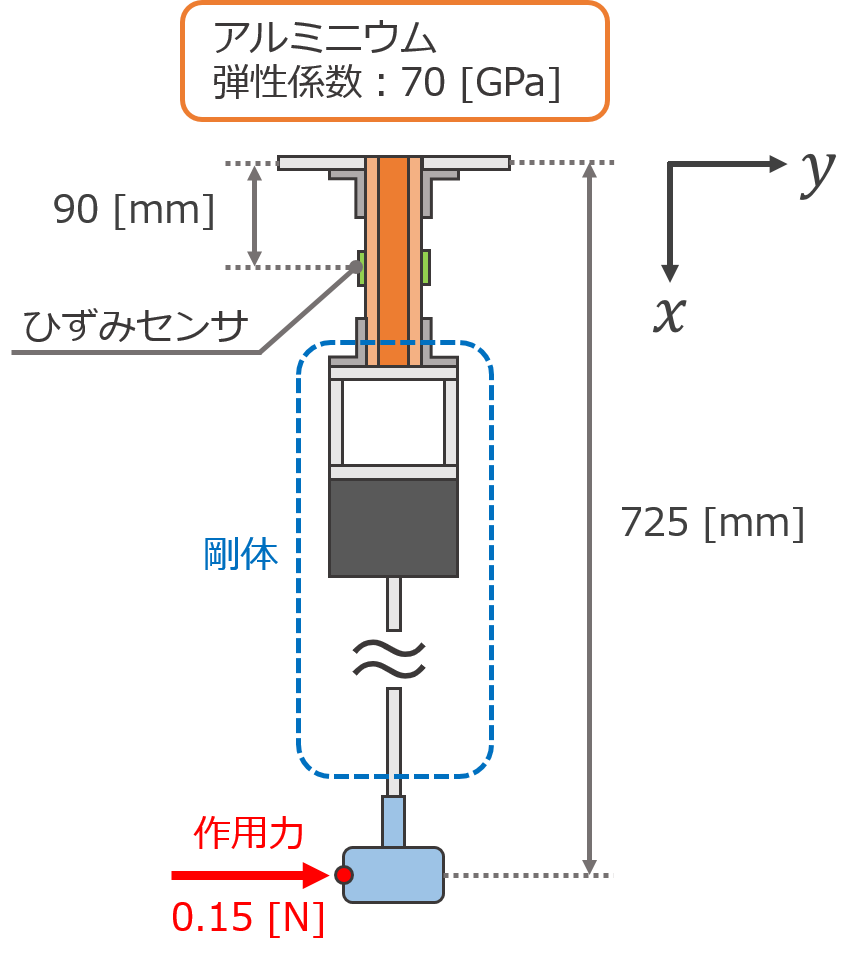
\includegraphics[width=70mm]{../images/moment.png}
        \caption{Cross-sectional shape of experimental device}
    \end{center}
\end{figure}

\subsubsection{算出過程}
\begin{itemize}
    \item [$\blacksquare$] 実験装置に加わるモーメントの算出
    \begin{eqnarray*}
        M &=& F × \frac{l_1}{1000}\\
        &=& 0.15 × 0.725\\
        &=& 0.10875 \;\left[\mathrm{N \cdot m}\right]
    \end{eqnarray*}
    \item [$\blacksquare$] たわみの曲率半径の算出
    \begin{itembox}[l]{たわみの曲率半径}
        \begin{center}
            $\displaystyle \frac{1}{R} = \frac{M}{EI}$
        \end{center}
    \end{itembox}
    \begin{eqnarray*}
        R &=& \frac{EI}{M}\\
        &=& 70 × 2701 × \frac{100000}{10875}\\
        &\approx& 1738577.713 \left[\mathrm{mm}\right]
    \end{eqnarray*}
    \item [$\blacksquare$] 位置$x$[mm] におけるたわみ角とたわみの算出
    \begin{itembox}[l]{たわみの微分方程式}
            \begin{center}
                $\displaystyle \frac{d^2w}{dx^2}=-\frac{M}{EI}$\\
                \vskip\baselineskip
                ※ 今回のひずみは正の値となる
            \end{center}
    \end{itembox}
    \begin{itembox}[l]{初期条件}
    \begin{itemize}
        \item [$\bullet$] $x=0$ のとき $w=0$,$\theta =0$
    \end{itemize}
    \end{itembox}
    \begin{eqnarray*}
        \frac{d^2w}{dx^2}&=&\frac{M}{EI}\\
        &=&\frac{0.10875}{70 × 2701}\\
        &=&5.7518 \cdots × 10^{-7}\\
        &\approx& 5.752 × 10^{-7} \;\left[\mathrm{1/mm}\right]\\ \\
        \frac{dw}{dx} &=& \theta = \frac{M}{EI} x + C_1\\ \\
        w &=& \frac{1}{2} \frac{M}{EI} x^2 + C_1x + C_2
    \end{eqnarray*}
    初期条件より
    \begin{eqnarray*}
        C_1 = C_2 = 0
    \end{eqnarray*}
    したがって,
    \begin{eqnarray*}
        \theta &=& \frac{M}{EI}x\\ \\
        w &=& \frac{1}{2}\frac{M}{EI}x^2\\
    \end{eqnarray*}
        \item [$\blacksquare$] ひずみセンサ取付部($x=90$)の伸びの算出\\
    $x = 90$のとき,たわみ角は,
    \begin{eqnarray*}
        \theta &=& \frac{M}{EI} × 90\\
        &=& 5.7152 × 10^{-7} × 90\\
        &=& 5.1437 × 10^{-5}\\
        &\approx& 5.144 × 10^{-5} \;\left[\mathrm{rad}\right]
    \end{eqnarray*}
    したがって,取付軸の伸び$\lambda$は,
    \begin{eqnarray*}
        \lambda &=& \left(R+\delta r\right)\theta - R\theta\\
        &=& \delta r \theta\\
        &=& 10 × \;\theta\\
        &=& 10 × 5.1437 × 10^{-5}\\
        &=& 5.1437 × 10^{-4}\\
        &\approx& 5.144 × 10^{-4} \;\left[\mathrm{mm}\right]\\
    \end{eqnarray*}
    \item [$\blacksquare$] ひずみセンサ取付部($x=90$)のひずみの算出
        \begin{eqnarray*}
            \varepsilon &=& \frac{\lambda}{l_2}\\
            &=& \frac{5.144 × 10^{-4}}{180}\\
            &=& 2.8577 × 10^{-6}\cdots\\
            &\approx& 2.858 × 10^{-6} \left[\mathrm{-}\right]
        \end{eqnarray*}
    \item [$\blacksquare$] 先端($x=725$)のたわみ量 $w$ の算出
    \begin{eqnarray*}
        w &=& \frac{1}{2} × \frac{M}{EI} × l^2\\
        &=& \frac{1}{2} × 5.752 × 10^{-7} × 725^2\\
        &=& 0.1511 \cdots\\
        &\approx& 0.151 \;\left[\mathrm{mm}\right]
    \end{eqnarray*}
\end{itemize}

\subsection{ひずみ量の算出式の作成}

\subsubsection{算出過程}
\begin{eqnarray*}
    \varepsilon &=& \frac{\lambda}{l_2}\\
    &=& \frac{\theta}{l_2} × \delta r\\
    &=& \frac{M × 90}{l_2 × EI} × \delta r\\
    &=& \frac{l_1 × 90}{1000 × l_2 × EI} × F × \delta r\\
    &=& \frac{725 × 90}{1000 × 180 × 70 × 2701} × F × \delta r\\
    &=& 1.9172 \cdots × 10^{-6} × F × \delta r\\
    &\approx& 1.917 × 10^{-6} × F × \delta r\\
\end{eqnarray*}

\begin{itembox}[l]{ひずみ量の算出式}
    \begin{center}
        $\displaystyle \varepsilon = 1.197 × 10^{-6} × F × \delta r$
    \end{center}
\end{itembox}

また,取付部表面と中立軸の距離:$\delta r$について
比較形状ごとの値を以下に示す.

% \begin{itembox}[l]{比較形状の寸法}
%     \begin{enumerate}[(i)]
%         \item 円筒 : $D_1=\;$20.0 [mm],$D_2=\;$18.0 [mm]
%         \item 円柱 : $D=\;$15.3 [mm]
%         \item 角柱 : $L=\;$13.4 [mm]
%     \end{enumerate}
% \end{itembox}

\begin{itembox}[l]{取付部表面と中立軸の距離}
    \begin{enumerate}[(i)]
        \item 円筒 : $\delta r_1 = 10.0$ [mm]
        \item 円柱 : $\delta r_2 = 7.65$ [mm]
        \item 角柱 : $\delta r_3 = 6.70$ [mm]
    \end{enumerate}
\end{itembox}

したがって,実験装置に加えられる作用力を 1 [N] と仮定し,
それぞれの比較形状についてひずみを算出すると,以下のようになる.

\begin{itembox}[l]{各試験片のひずみ量}
    \begin{enumerate}[(i)]
        \item 円筒 : $\varepsilon_1 \approx 1.197 × 10^{-5}$ [-]
        \item 円柱 : $\varepsilon_2 \approx 1.467 × 10^{-5}$ [-]
        \item 角柱 : $\varepsilon_3 \approx 1.284 × 10^{-5}$ [-]
    \end{enumerate}
\end{itembox}

\newpage

\section{ひずみゲージの選定}

\subsection{現在使用しているロードセルについて}
現在使用しているロードセルについての情報を以下に示す。
\begin{screen}
    \begin{itemize}
        \item [$\bullet$]   名称  : 微小荷重圧縮引張型 UTA
        \item [$\bullet$]   型番  : UTA-100GR
        \item [$\bullet$]  定格容量 : $0.9807 ~ 19.61 \left[\mathrm{N}\right]$
        \item [$\bullet$] 推奨印可電圧: 3V 以下
    \end{itemize}
\end{screen}

\end{document}